\section{Adeline} \label{sc:adel}

\subsection{Aufbau}

In 1959 entwickelten der Stanford Professor Bernard Widrow und der Elektroingenieur Marcian Edward Hoff das sogenannte \emph{Adeline-Modell}. Der Name ist ein Akronym für \emph{ADAptive LINear Element}. Dieses Modell basiert auf dem Perceptron mit dem Unterschied, dass dieses Modell auf die Einheits-Sprungfunktion, wie sie das Peceptron bei der Angleichung der Gewichte verwendet, verzichtet. Es wird stattdessen eine lineare Aktivierungsfunktion ${g(z)}$ verwendet, welche in diesem Fall erstmal mit der Identitätsfunktion besetzt wird (es gilt also ${g(w^Tx) = w^Tx}$). Außerdem wird eine Entscheidungsfunktion an das Ende des ganzen Modells gehängt um weiterhin die Werte quantifizieren zu können. Diese hat jedoch keinen Einfluss auf den Trainingsalgorithmus. 

\begin{figure}[!htb]
	\centering
	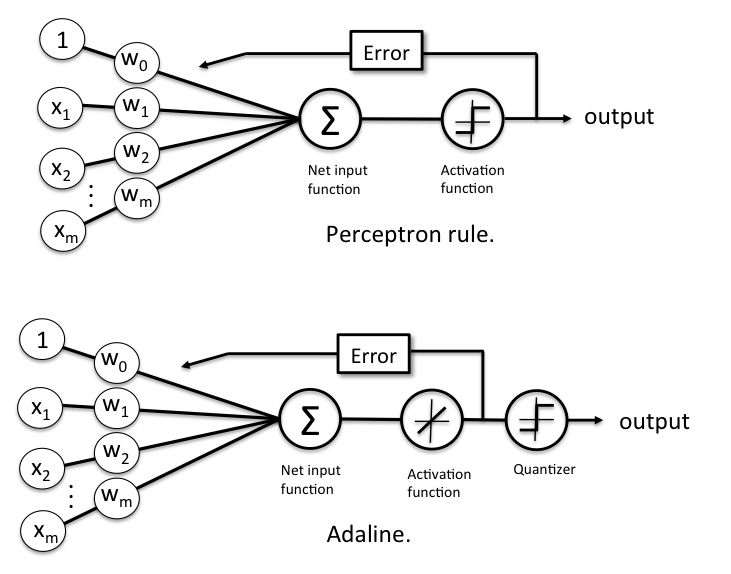
\includegraphics[width=.8\linewidth]{img/adeline_aufbau}
	\mycaption{Adeline - Aufbau}{mpNeuron}
	\label{fig:ad_aufbau}
\end{figure}


\subsection{Lernalgorithmus} \label{ss:la}

Widrow und Hoff definierten die Delta-Regel für den Lernalgorithmus ihres Modells. Dieser ist auch unter dem Namen \emph{Least-Mean-Square-Algorithmus} bekannt und ist auch heute noch von Relevanz. Im Kern möchte man hierbei das Minimum einer Kostenfunktion über dem Modell bestimmen. Ich werde im folgenden Abschnitt darauf eingehen, wie, dieser funktioniert und wie genau er für dieses Modell eingesetzt werden kann. 

\paragraph{Gradientenverfahren}
Der wesentliche Nachteil der Einheits-Sprungfunktion ist der, dass sie nicht stetig und damit auch nicht differenzierbar ist. Deswegen hat man sich beim Lernalgorithmus des Adeline-Modells dazu entschieden stattdessen die Identitätsfunktion zu verwenden. 

Es wird zuerst eine Kostenfunktion ${J(w)}$ definiert die minimiert werden soll. Die Kostenfunktion wird durch die \emph{Regressionsquadratsumme}\footnote{engl. \emph{sum of squared errors} (SSE)} definiert. Die Formel sieht folgendermaßen aus: 

\begin{equation}
J(w)  = \frac{1}{2} \sum_{i} (\text{target}^{(i)} - \text{output}^{(i)})^2 \quad \quad \text{output}^{(i)} \in \mathbb{R} \\
\end{equation}

Wichtig hierbei, der Vorfaktor ${ \frac{1}{2} }$ gehört nicht zur herkömmlichen Regressionsquadratsumme, wurde hier jedoch hinzugefügt um später einfacher ableiten zu können. Ziel ist es die bestimmte Abweichung über alle Trainingsdaten so minimal wie möglich zu gestalten. Dazu muss man die Gewichte sowie die Schwellwerte entsprechend anpassen. Um das zu tun, reicht es das Minimum dieser Funktion zu finden. Dazu bedient man sich einer Technik namens \emph{Gradientenverfahren} (englisch \emph{gradient descent}). 

Werfen wir einen Blick auf die Abbildung \ref{fig:ad_gd1}. 

\begin{figure}[!htb]
	\centering
	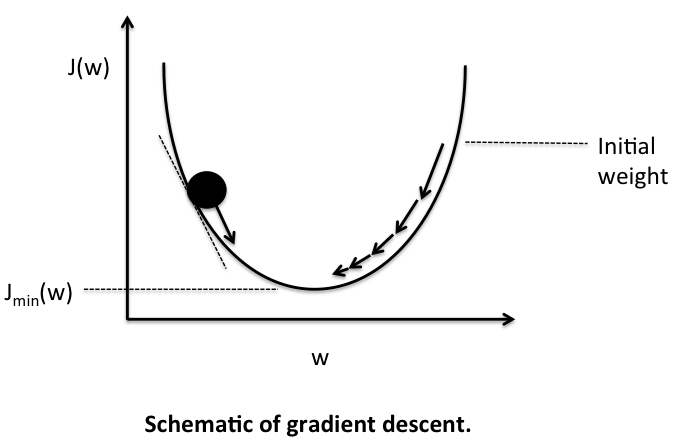
\includegraphics[width=.7\linewidth]{img/adeline_gd1}
	\mycaption{Gradientenverfahren mit eindimensionaler Kostenfunktion}{mpNeuron}
	\label{fig:ad_gd1}
\end{figure}

Die dargestellte Funktion besitzt nur einen Eingabewert. Zur Veranschaulichung kann man sich einen Ball vorstellen, der einen Berg bzw. in ein Tal herunter rollt. Bezogen auf das Beispiel betrachtet man einen einen beliebigen Funktionswert und bestimmt die Ableitung an dieser Stelle. Diese Ableitung kann auch als \glqq Steigung\grqq  an der betrachteten Stelle verstanden werden. Wenn man diese nun invertiert hat, bekommt man theoretisch die \glqq Richtung\grqq  in die der Ball rollen müsste. Ähnlich wie schon der Lernalgorithmus beim Perceptron, wird mit einer Lernrate ${\eta}$ gearbeitet, die bestimmt wie viel Veränderung in einem Iterations-Schritt stattfinden soll. Im Beispiel könnte man diese als Schrittweite verstehen. 
Wie weit in einem Schritt gearbeitet wird, ist von fundamentaler Bedeutung. In Abbildung \ref{fig:ad_gd2} ist zu sehen, dass es problematisch sein kann die Lernrate zu hoch zu definieren, denn der Algorithmus kann das Minimum auch überspringen. Andererseits kann es auch zu Problemen kommen wenn die Lernrate zu klein definiert wurde, da der Algorithmus eventuell in einem lokalen Minimum \glqq steckenbleibt\grqq . Um gerade das erste Problem zu beheben wird die Lernrate heutzutage in jedem Iterationsschritt in Abhängigkeit der Größe der Steigung berechnet.

\begin{figure}[!htb]
	\centering
	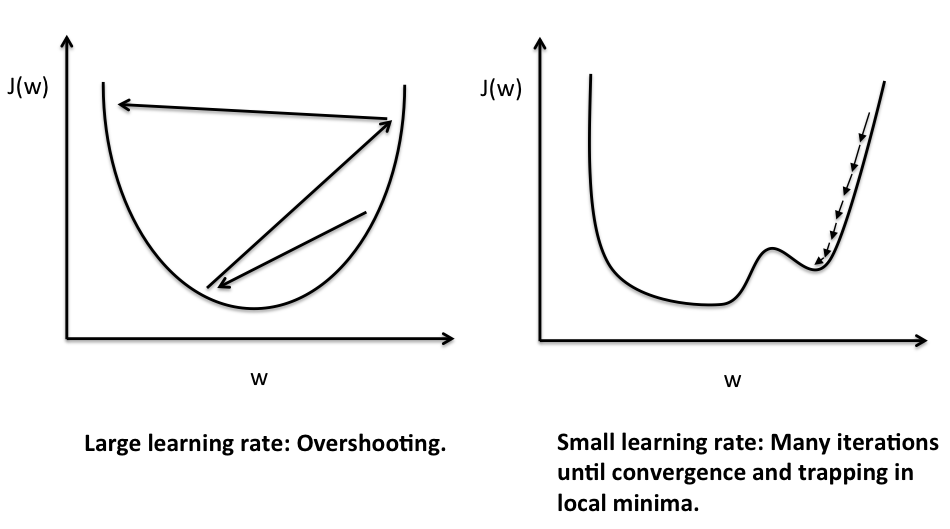
\includegraphics[width=\linewidth]{img/adeline_learning_rate}
	\mycaption{Gradientenverfahren - unterschiedliche Lernraten}{mpNeuron}
	\label{fig:ad_gd2}
\end{figure}

Letztendlich besitzt das hier betrachtete Modell aber meist mehr als ein einzelnes Gewicht, weswegen man sich nun damit auseinander setzen muss, wie man dieses Verfahren auf eine Kostenfunktion mit einem mehrdimensionalen Vektor anpassen muss. Mit einem zweidimensionalen Eingabevektor ist dies noch relativ gut darstellbar (siehe Abbildung \ref{fig:ad_gd3}).

\begin{figure}[!htb]
	\centering
	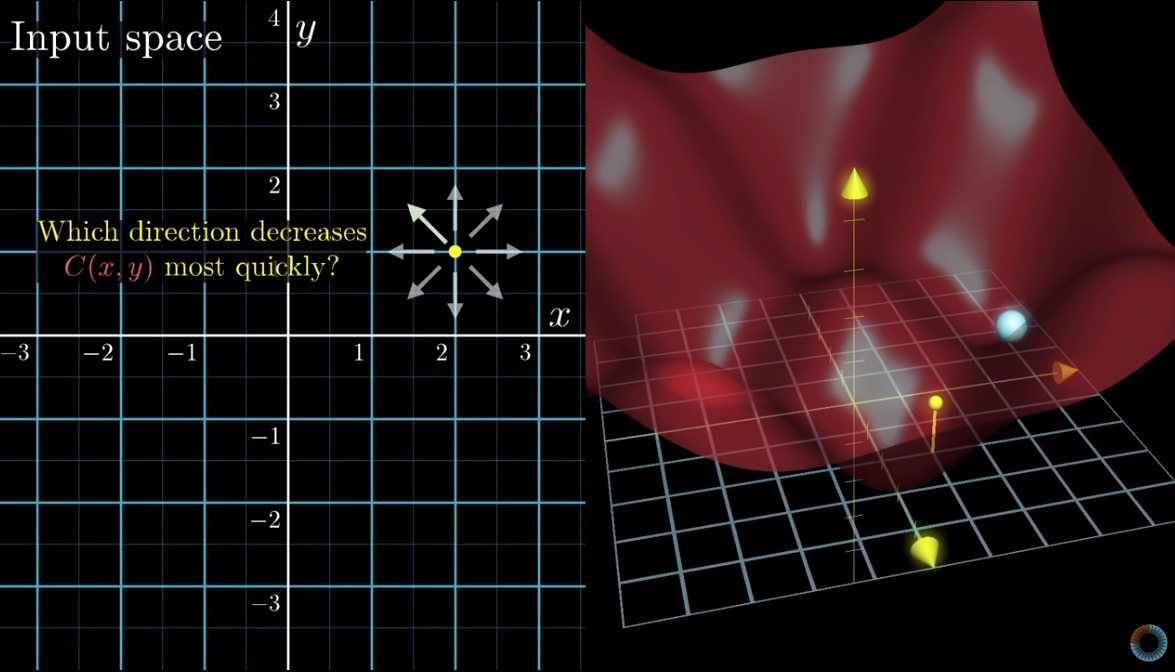
\includegraphics[width=\linewidth]{img/3dPlot_1}
	\mycaption{Gradientenverfahren - zweidimensionaler Eingabevektor}{mpNeuron}
	\label{fig:ad_gd3}
\end{figure}

Auch bei Funktionen mit mehreren Eingabewerten ist es möglich an einem betrachteten Eingabevektor die Steigung zu bestimmen. Allgemein wird diese als \emph{Gradientenvektor} bezeichnet. Bei der gerade betrachteten Abbildung bilden die \emph{x}- und die \emph{y-Achse} jeweils die beiden Eingabewerte der Funktion, wobei die Ausgabe mit der \emph{z-Achse} dargestellt wird. Hier wird die Analogie mit dem Herabrollen eines Berges vielleicht noch etwas klarer. Auch hier gilt, wie  schon bei den anderen betrachteten Modellen, wieder die Notation: 

\begin{equation} \label{eq:gewupd}
{w = w + \Delta w}
\end{equation}

${\Delta w}$ stellt den angedeuteten Gradientenvektor dar. Im mehrdimensionalen Raum ist diese Gewichtsveränderung im allgemeinen Fall den kompletten Gewichtsvektor und für den speziellen Fall mit einem einzelnen Gewicht folgendermaßen definiert. 

\vspace{3mm}
\begin{mytheo}{Gradient}{theoexample} \label{theo:gradient1}
Allgemein: 
\begin{equation}
{\Delta w = - \eta \nabla J(w)}
\end{equation}

Für die jeweiligen Gewichte: 
\begin{equation}
\Delta w_j = - \eta \frac{\partial J}{\partial w_j}
\end{equation}

\end{mytheo}

\subparagraph{Exkurs - Partielle Ableitungen \cite{partAbl}}
Da es sich im Beispiel um einen mehrdimensionalen Eingabevektor handelt, muss man mit den partiellen Ableitungen arbeiten. Diese lassen sich am besten anhand eines weiteren Beispiels erklären. Betrachten wir zuerst einmal die Funktion ${{f(x, y) = x^2 + y^2}}$ (siehe Abbildung \ref{fig:partAbl1}). 

\begin{figure}[!htb]
	\centering
	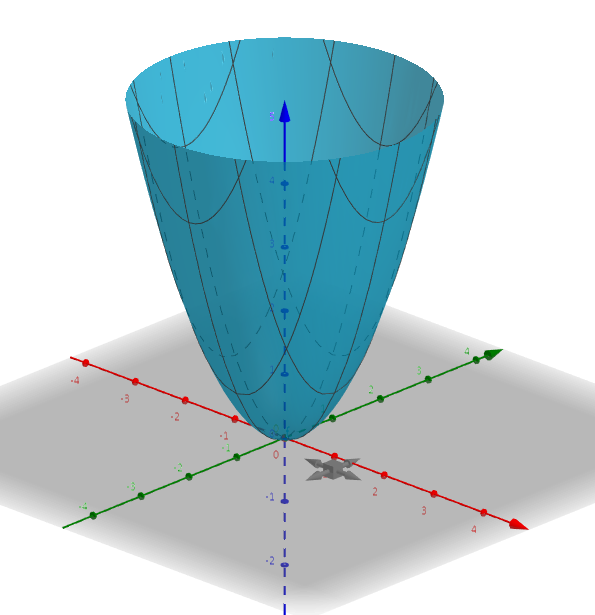
\includegraphics[width=.6\linewidth]{img/partAbl_1}
	\caption[Partielle Ableitung 1]{Partielle Ableitung 1 \protect\footnotemark}
	\label{fig:partAbl1}
\end{figure}

\FloatBarrier
\footnotetext{Mit Geogebra 3d erstellt: \url{https://www.geogebra.org/3d}}

Wann man nun einen Punkt auf der Oberfläche der Funktion betrachtet ist es nicht möglich zu sagen wie stark die Steigung ist, denn es fehlt eine Richtung bezüglich der \glqq geschaut\grqq  werden soll. Hierzu betrachten wir noch einmal die Abbildung \ref{fig:partAbl2}. Hier wurde eine \glqq rote Ebene \glqq eingeführt. Dies kann als \emph{Blickwinkel} angesehen werden. Wenn man nun einen Punkt auf dieser Schnittgerade betrachtet ist es möglich die zugehörigen Steigung zu ermitteln. Um die Ebene in der betrachteten Abbildung zu erzeugen wird einfach eine der beiden Eingabeparameter auf einen Wert festgelegt (in diesem Fall ${y=1}$). Man kann natürlich auch den Wert für den Eingabeparameter \emph{x} festlegen und \emph{y} als Laufvariable betrachten. 

Dieser Prozess des Aufteilens der Ableitungen in die einzelnen Teile wird als \emph{Partiale Ableitung} bezeichnet. Wir nehmen eine Funktion mit mehrdimensionalem Eingabevektor und berechnen für jede Komponente des Vektors die Ableitung. Kurze Anmerkung zur Notation: Im Zähler des Bruchs welcher die Partielle Ableitung angibt steht stets die Funktion welche abgeleitet werden soll, während man im Nenner die Variable bezüglich der abgeleitet werden soll notiert.


\begin{minipage}{\linewidth}
In unserem Beispiel besitzt die Funktion ${ z = f(x, y) = x^2 + y^2 }$ folgende Ableitung: 

\begin{equation}
\begin{aligned}
& z = f(x, y) = x^2 + y^2 \\
& \frac{\partial z}{\partial x} = 2x \\
& \frac{\partial z}{\partial y} = 2y \\
\end{aligned}
\end{equation}

\end{minipage}

Um nun den Gradienten zu bestimmen muss man diese einfach nur aufaddieren: 

\begin{equation}
  \Delta J \approx \frac{\partial J}{\partial w_1} \Delta w_1 +
  \frac{\partial J}{\partial w_2} \Delta w_2.
\end{equation}

\begin{figure}%
  \centering
  \subfloat[][]{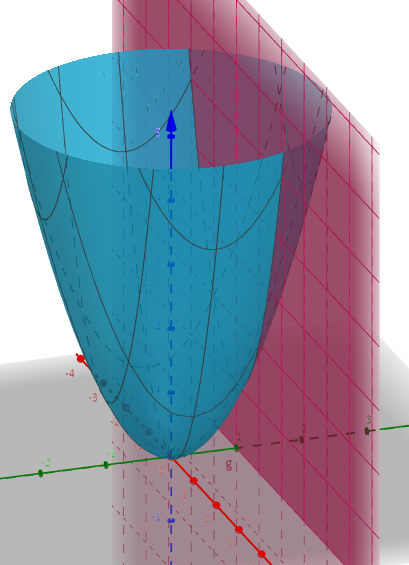
\includegraphics[width=.4\linewidth]{img/partAbl_2}}
  \qquad
  \subfloat[][]{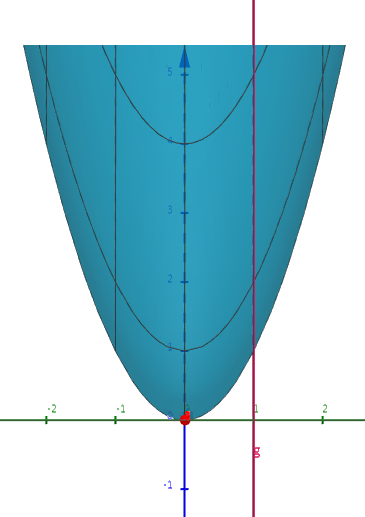
\includegraphics[width=.4\linewidth]{img/partAbl_3}}
  \caption{Partielle Ableitung 2}
  \label{fig:partAbl2}
\end{figure}


\vspace{1cm}

\subparagraph{Batch-Gradientenabstieg}
Um den Gradientenvektor der Kostenfunktion (Regressionsquadratsumme) zu bestimmen greift folgender Formelapparat welchen ich im folgenden schrittweise durchgehen werde.

\vspace{2 mm}
\begin{minipage}{\textwidth}
\begin{myderivation}{Gradient}{theoexample} \label{deri:grad}

\begin{equation} \label{eq:gr1}
\frac{\partial J}{\partial w_j} = \frac{\partial }{\partial w_j} \frac{1}{2} \sum_i  (t^{(i)} - o^{(i)})^2 \\
\end{equation}

\begin{equation} \label{eq:gr2}
\frac{\partial J}{\partial w_j} = \frac{1}{2} \sum_i \frac{\partial }{\partial w_j} (t^{(i)} - o^{(i)})^2 \\
\end{equation}

\begin{equation} \label{eq:gr3}
\frac{\partial J}{\partial w_j} = \frac{1}{2} \sum_i 2 (t^{(i)} - o^{(i)}) \frac{\partial }{\partial w_j} (t^{(i)} - o^{(i)}) \\
\end{equation}

\begin{equation} \label{eq:gr4}
\frac{\partial J}{\partial w_j} = \sum_i (t^{(i)} - o^{(i)}) \frac{\partial }{\partial w_j} \bigg(t^{(i)} - \sum_j w_j x^{(i)}_{j}\bigg) \\
\end{equation}

\begin{equation} \label{eq:gr5}
\frac{\partial J}{\partial w_j} = \sum_i  (t^{(i)} - o^{(i)})(-x^{(i)}_{j})
\end{equation}

\end{myderivation}
\end{minipage}


\begin{enumerate}

\item Gleichung \ref{eq:gr1}: Da wir den Gradienten der Kostenfunktion (Regressionsquadratsumme) bilden wollen müssen wir diese bezüglich des gerade betrachteten Gewichts ableiten. Deswegen notiert man im Zähler die Funktion \emph{J} auf der linken Seite der Gleichung und schreibt sie auf der rechten Seite einfach einmal aus. Im Nenner befindet sich das Gewicht an der Stelle $j$. 

\item Gleichung \ref{eq:gr2}: Die Summe sowie der Faktor $\frac{1}{2}$ kann generell aus der Ableitung rausgezogen werden ohne etwas am Gesamtergebnis zu verändern. 

\item Gleichung \ref{eq:gr3}: Ein erster Ableitungssschritt bezüglich der Kettenregel wird angewandt. Die äußere Funktion $ 2 (t^{(i)} - o^{(i)}) $ wird vor die noch ausstehende Ableitung der inneren Funktion $  \frac{\partial }{\partial w_j} (t^{(i)} - o^{(i)}) $ gehängt. 

\item Gleichung \ref{eq:gr4}: Der konstante Faktor $2$ wird aus der Summe herausgezogen und direkt mit dem am Anfang hinzugefügten Faktor $ \frac{1}{2} $ multipliziert. Außerdem wird die eigentliche Berechnung der Ausgabe für $ o^{(i)} $ eingesetzt ($\sum_j w_j x^{(i)}_{j}$). 

\item Gleichung \ref{eq:gr5}: Es wird die innere Ableitung nach dem Gewicht $w_j$ gebildet. Das $t^{(i)}$ entfällt, da es sich um einen konstanten Faktor handelt. Der Faktor $-1$ kann vorgezogen werden womit man nur noch die Summe $ \sum_j w_j x^{(i)}_{j} $ ableiten muss. Wie bereits beim Perceptron (siehe Gleichung \ref{eq:vektorprod}) bildet sich die letztendliche Ausgabe ja über das Vektorprodukt ${w^Tx}$. Wenn man die Summe ausschreibt fällt einem auf, dass es nur einen einzigen Term in der kompletten Summe gibt welcher den Faktor $w_j$ beinhaltet über welchem hier schließlich abgeleitet werden soll. Daher Ist es möglich die gesamte Summe auf $-x^{(i)}_{j}$ abzuleiten. 

\end{enumerate}

\begin{mytheo}{Gradient}{theoexample}

Gradientenkomponente: 
\begin{equation}
\frac{\partial J}{\partial w_j} = \sum_i  (t^{(i)} - o^{(i)})(-x^{(i)}_{j})
\end{equation}

Dies muss nun in die ursprüngliche Form (siehe Gleichung \ref{theo:gradient1} Seite \pageref{theo:gradient1}) eingefügt werden: 
\begin{equation}
\Delta w_j = - \eta \frac{\partial J}{\partial w_j} = - \eta \sum_i  (t^{(i)} - o^{(i)})(- x^{(i)}_{j}) = \eta \sum_i (t^{(i)} - o^{(i)})x^{(i)}_{j}
\end{equation}

Der komplette Gradientenvektor beinhaltet die Ergebnisse für die Ableitungsschritte nach jedem einzelnen Gewicht:
\begin{equation}
  \nabla J \equiv \left(\frac{\partial J}{\partial w_1}, \ldots, 
  \frac{\partial J}{\partial w_m}\right)^T.
\end{equation}

\end{mytheo}

Die einzelnen Komponenten des Gradientenvektors können dann wieder mit der allererste Formel (siehe Gleichung  \ref{eq:gewupd}) in neue Gewichte verrechnet werden. 

Die wesentlichen Unterschiede zum Lernalgorithmus, welcher beim Perceptron verwendet wird, bestehen daraus, dass der Ausgabewert bei diesem Modell mit einer reellen Zahl dargestellt wird. Außerdem wird für das Aktualisieren eines Gewichts die komplette Menge an Trainingsdatensätzen verwendet. Deswegen wird diese Herangehensweise auch \emph{Batch-Gradientenabstieg} genannt. Beim Perceptron wird das Gewicht nach jedem einzelnen Trainingsdatensatz gerichtet. Eine Implementierung dieses Algorithmus befindet sich ebenfalls in dem Github Repository \cite{pcImplementierung}. 

\paragraph{Stochastischer Gradientenabstieg} \label{par:stochGA}
Der vorgestellte Algorithmus ist in der Praxis aber relativ rechenaufwendig weil man für jeden einzelnen Iterationsschritt alle Trainingsdatensätze betrachten muss. Ein Weg dies zu umgehen ist der sogenannte \emph{Mini-Batch Gradientenabstieg}. Hierbei wird die komplette Menge an Traininngsdatensätzen erst einmal gemischt und anschließend in kleinere Mengen unterteilt. Beim Iterationsschritt wird dann jeweils eine solcher Mengen betrachtet. Dies ist nicht der effizienteste Weg allerdings ist dieser viel schneller berechnet, dennoch gibt er eine gute Annäherung dafür wie die einzelnen Gewichte geändert werden müssen. In Abbildung \ref{fig:ad_gd4} kann man erkennen wie die unterschiedlichen Arten des Gradientenabstiegs grob arbeiten. Der linke Graph beschreibt den \glqq herkömmlichenlichen\grqq  Batch-Gradientenabstieg während der rechte den stochastischen darstellt. Dieser trifft zwar nie die genau Richtung ist allerdings immer relativ nah dran und findet letztendlich ebenfalls das Ziel. 

\begin{figure}[!htb]
	\centering
	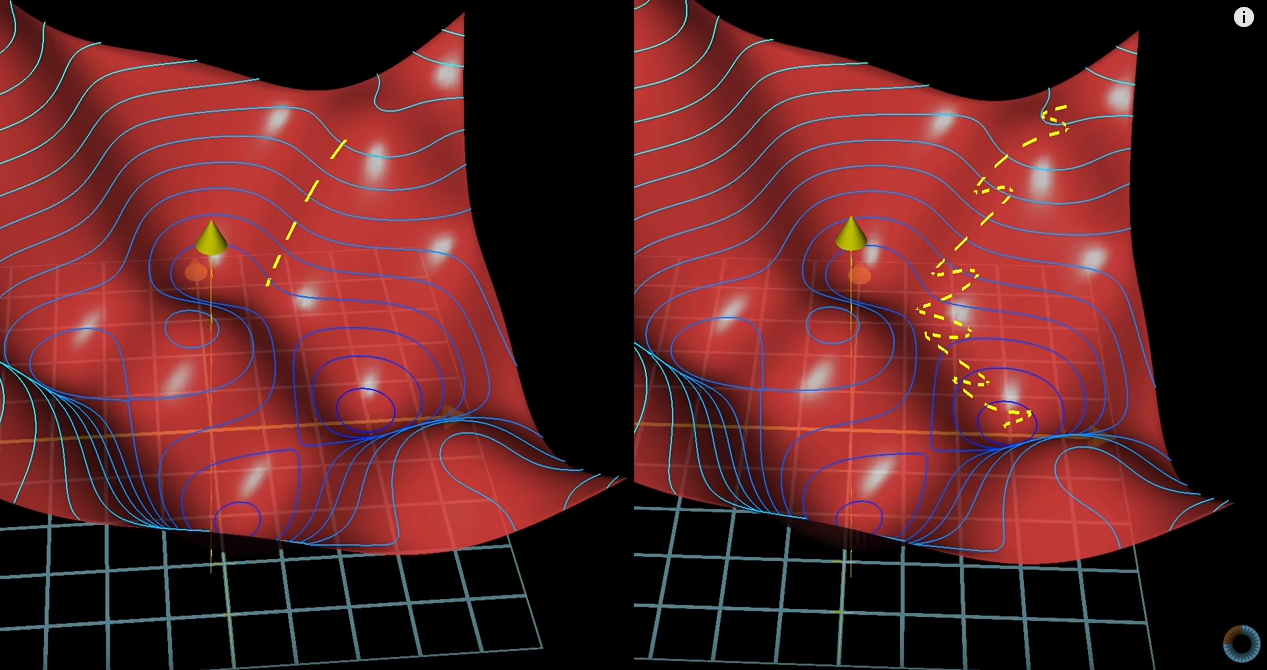
\includegraphics[width=\linewidth]{img/3dPlot_sgd}
	\mycaption{Gradientenverfahren - Vergleich}{3b1b}
	\label{fig:ad_gd4}
\end{figure}
